\documentclass[10pt, a4paper]{beamer}

\usetheme{Berkeley}
\usecolortheme{sidebartab}
\usepackage{graphicx}
\usepackage[utf8]{inputenc}
\usepackage[english]{babel}
 
\usepackage{hyperref}
\hypersetup{
    colorlinks=true,
    linkcolor=blue,
    filecolor=magenta,      
    urlcolor=cyan,
}
%\graphicspath{ {images/} }


\begin{document}
	\setbeamertemplate{sidebar left}{}
	\title{Progress Presentation-I}
	\subtitle{e-Yantra Summer Intership-2016 \\ Navigation In Indoor Environment Using AR Drone 2}
	\author{Balaji Gorantla\\Ridhwan Luthra\\
	Mentor: Vamshi, Simranjeet}
	\institute{IIT Bombay}
	\date{\today}
	%\addtobeamertemplate{sidebar left}{}{\includegraphics[scale = 0.3]{logowithtext.png}}
	\frame{\titlepage}

\setbeamertemplate{sidebar left}[sidebar theme]

\section{Overview of Project}
\begin{frame}{Overview of Project}
	Give following details: \\
	\begin{itemize}
		\item Project Name - Navigation In Indoor Environment Using AR Drone 2
		\item Objective - Given the map of the environment, make the drone navigate from one point to another. In simulation and in real world.
		\item Deliverables - Code and Documentation for each task, Video tutorial explaining each task.
	\end{itemize}
\end{frame}

\section{Parrot AR Drone 2.0}
\begin{frame}{Overview of Project}
	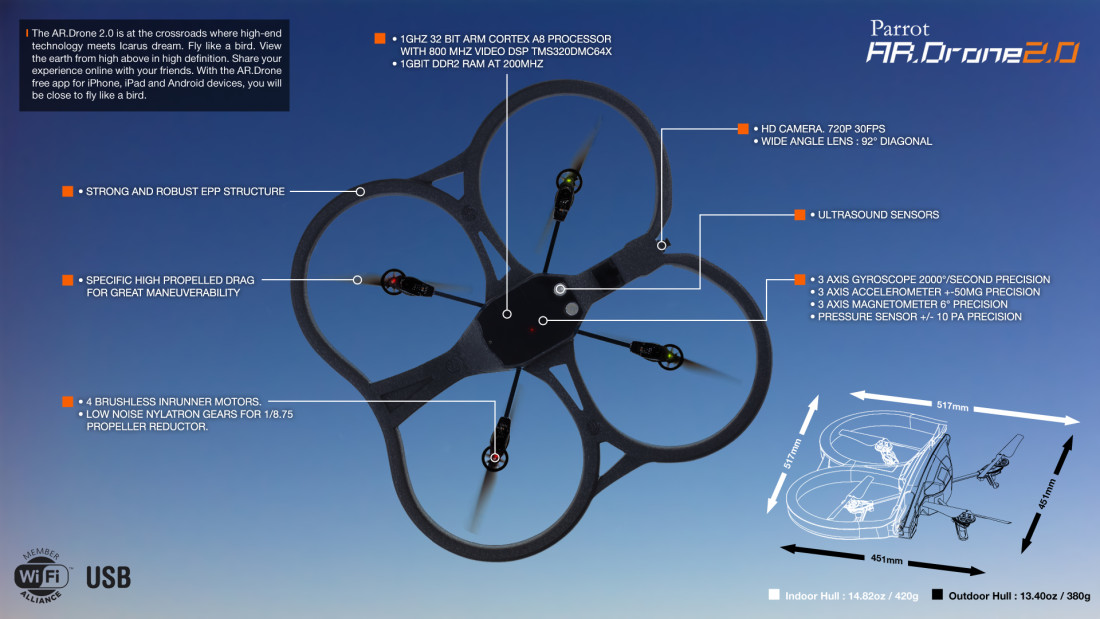
\includegraphics[scale=0.265]{drone_specs}
\end{frame}

\section{Overview of Task}
\begin{frame}{Overview of Task}
	\begin{table}[]
\centering
\begin{tabular}{|l|l|}
\hline
\textbf{Tasks}                                                                                          & \textbf{Deadline} \\ \hline
Setup environment                                                                             & 2 days   \\ \hline
Align drone to an ArUco marker in simulation                  & 6 days   \\ 
and real world (PID for 4 axis)                  &          \\ \hline
Generate 3D environment using Octomap                                                         & 2 days   \\ \hline
Spawn the quadrotor model, 3D map in RVIZ                     & 2 days   \\ 
and make it emulate a real one.                     &    \\ \hline
Literature Review on autonomous navigation                                                     & 2 days   \\ \hline
Autonomously navigate from 1 point to another                                                 & 6 days   \\ \hline
Generate a world in simulation in accordance to the room                                      & 2 days   \\ \hline
Generate a map with the world in simulation                                                   & 2 days   \\ \hline
Make the physical drone go in sync with the & 6 days   \\ 
simulated one in the shortest path. Reduce drift. &    \\ \hline
Project report                                                                                & 5 days   \\ \hline
\end{tabular}
\caption{overview of tasks}
\end{table}
\end{frame}

\section{Task Accomplished}
\begin{frame}{Task Accomplished}
	\begin{itemize}
		\item Environment setup
        \begin{itemize}
        	\item Install Ubuntu 14.04 and setup ROS, ardrone drivers, simulators, etc.
        \end{itemize}
    	\item Align AR drone to an ArUco marker
        \begin{itemize}
        	\item Getting the robot pose from the ArUco marker.
            \item PID tuning to keep the drone at a fixed location
        \end{itemize}
        \item Generate 3D map using octomap.
        \begin{itemize}
        	\item Using octomap server to load a .ot/.bt file and visualize it in Rviz.
        \end{itemize}
        \item Spawn quadrotor model, 3d map in Rviz and make it emulate a real one.
        \begin{itemize}
        	\item Visualizing the 3D map in Rviz.
            \item Spawn the quadrotor and fix transforms to make it emulate the real drone.
            \item Setup transforms between the map and the drone.
        \end{itemize}
		\item Included images/demo of accomplished work
	\end{itemize}
\end{frame}
\begin{frame}{Task Accomplished}
\begin{center}
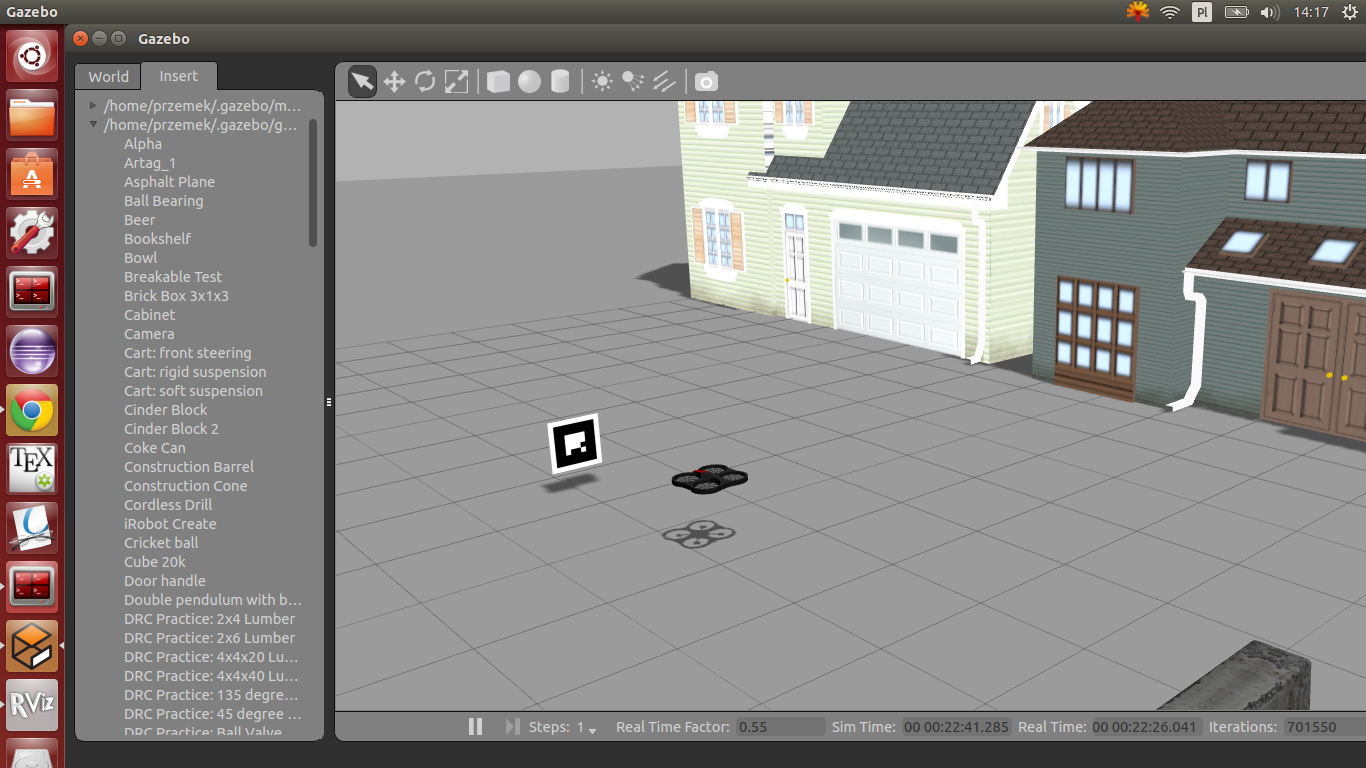
\includegraphics[scale=0.2]{aruco_align}\\
		Alignment of AR Drone with ArUco marker
\end{center}
		
\end{frame}
\begin{frame}{Task Accomplished}
\begin{center}
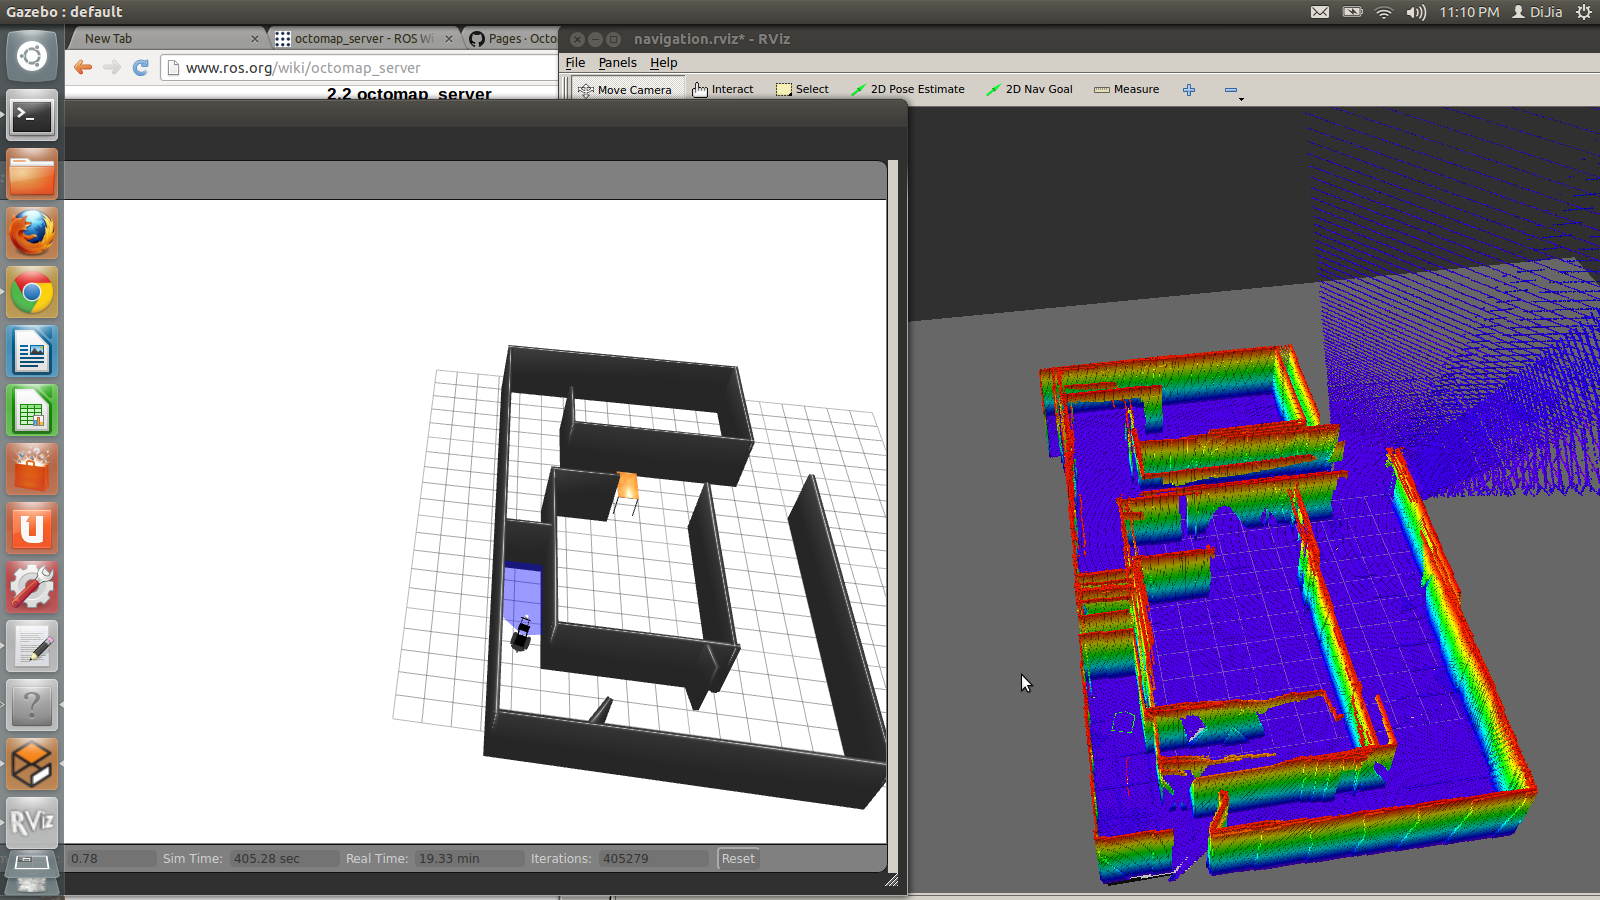
\includegraphics[scale=0.18]{octomap}\\
		3D map generated using octomap
\end{center}	
\end{frame}

\begin{frame}{Task Accomplished}
	\begin{itemize}
        \item 3D mapping in simulation
        \begin{itemize}
        	\item Using a turtlebot and octomap to create a 3D map of a world in simulation.
            \item Real time visualization of mapping in Rviz.
        \end{itemize}
        \item Literature Review of Autonomous navigation
        \begin{itemize}
        	\item Go through various research papers on autonomous navigation and decide what to use.
        \end{itemize}
        \item Documentation completed for tasks accomplished.
		\item Included images/demo of accomplished work
	\end{itemize}
\end{frame}

\begin{frame}{Task Accomplished}
\begin{center}
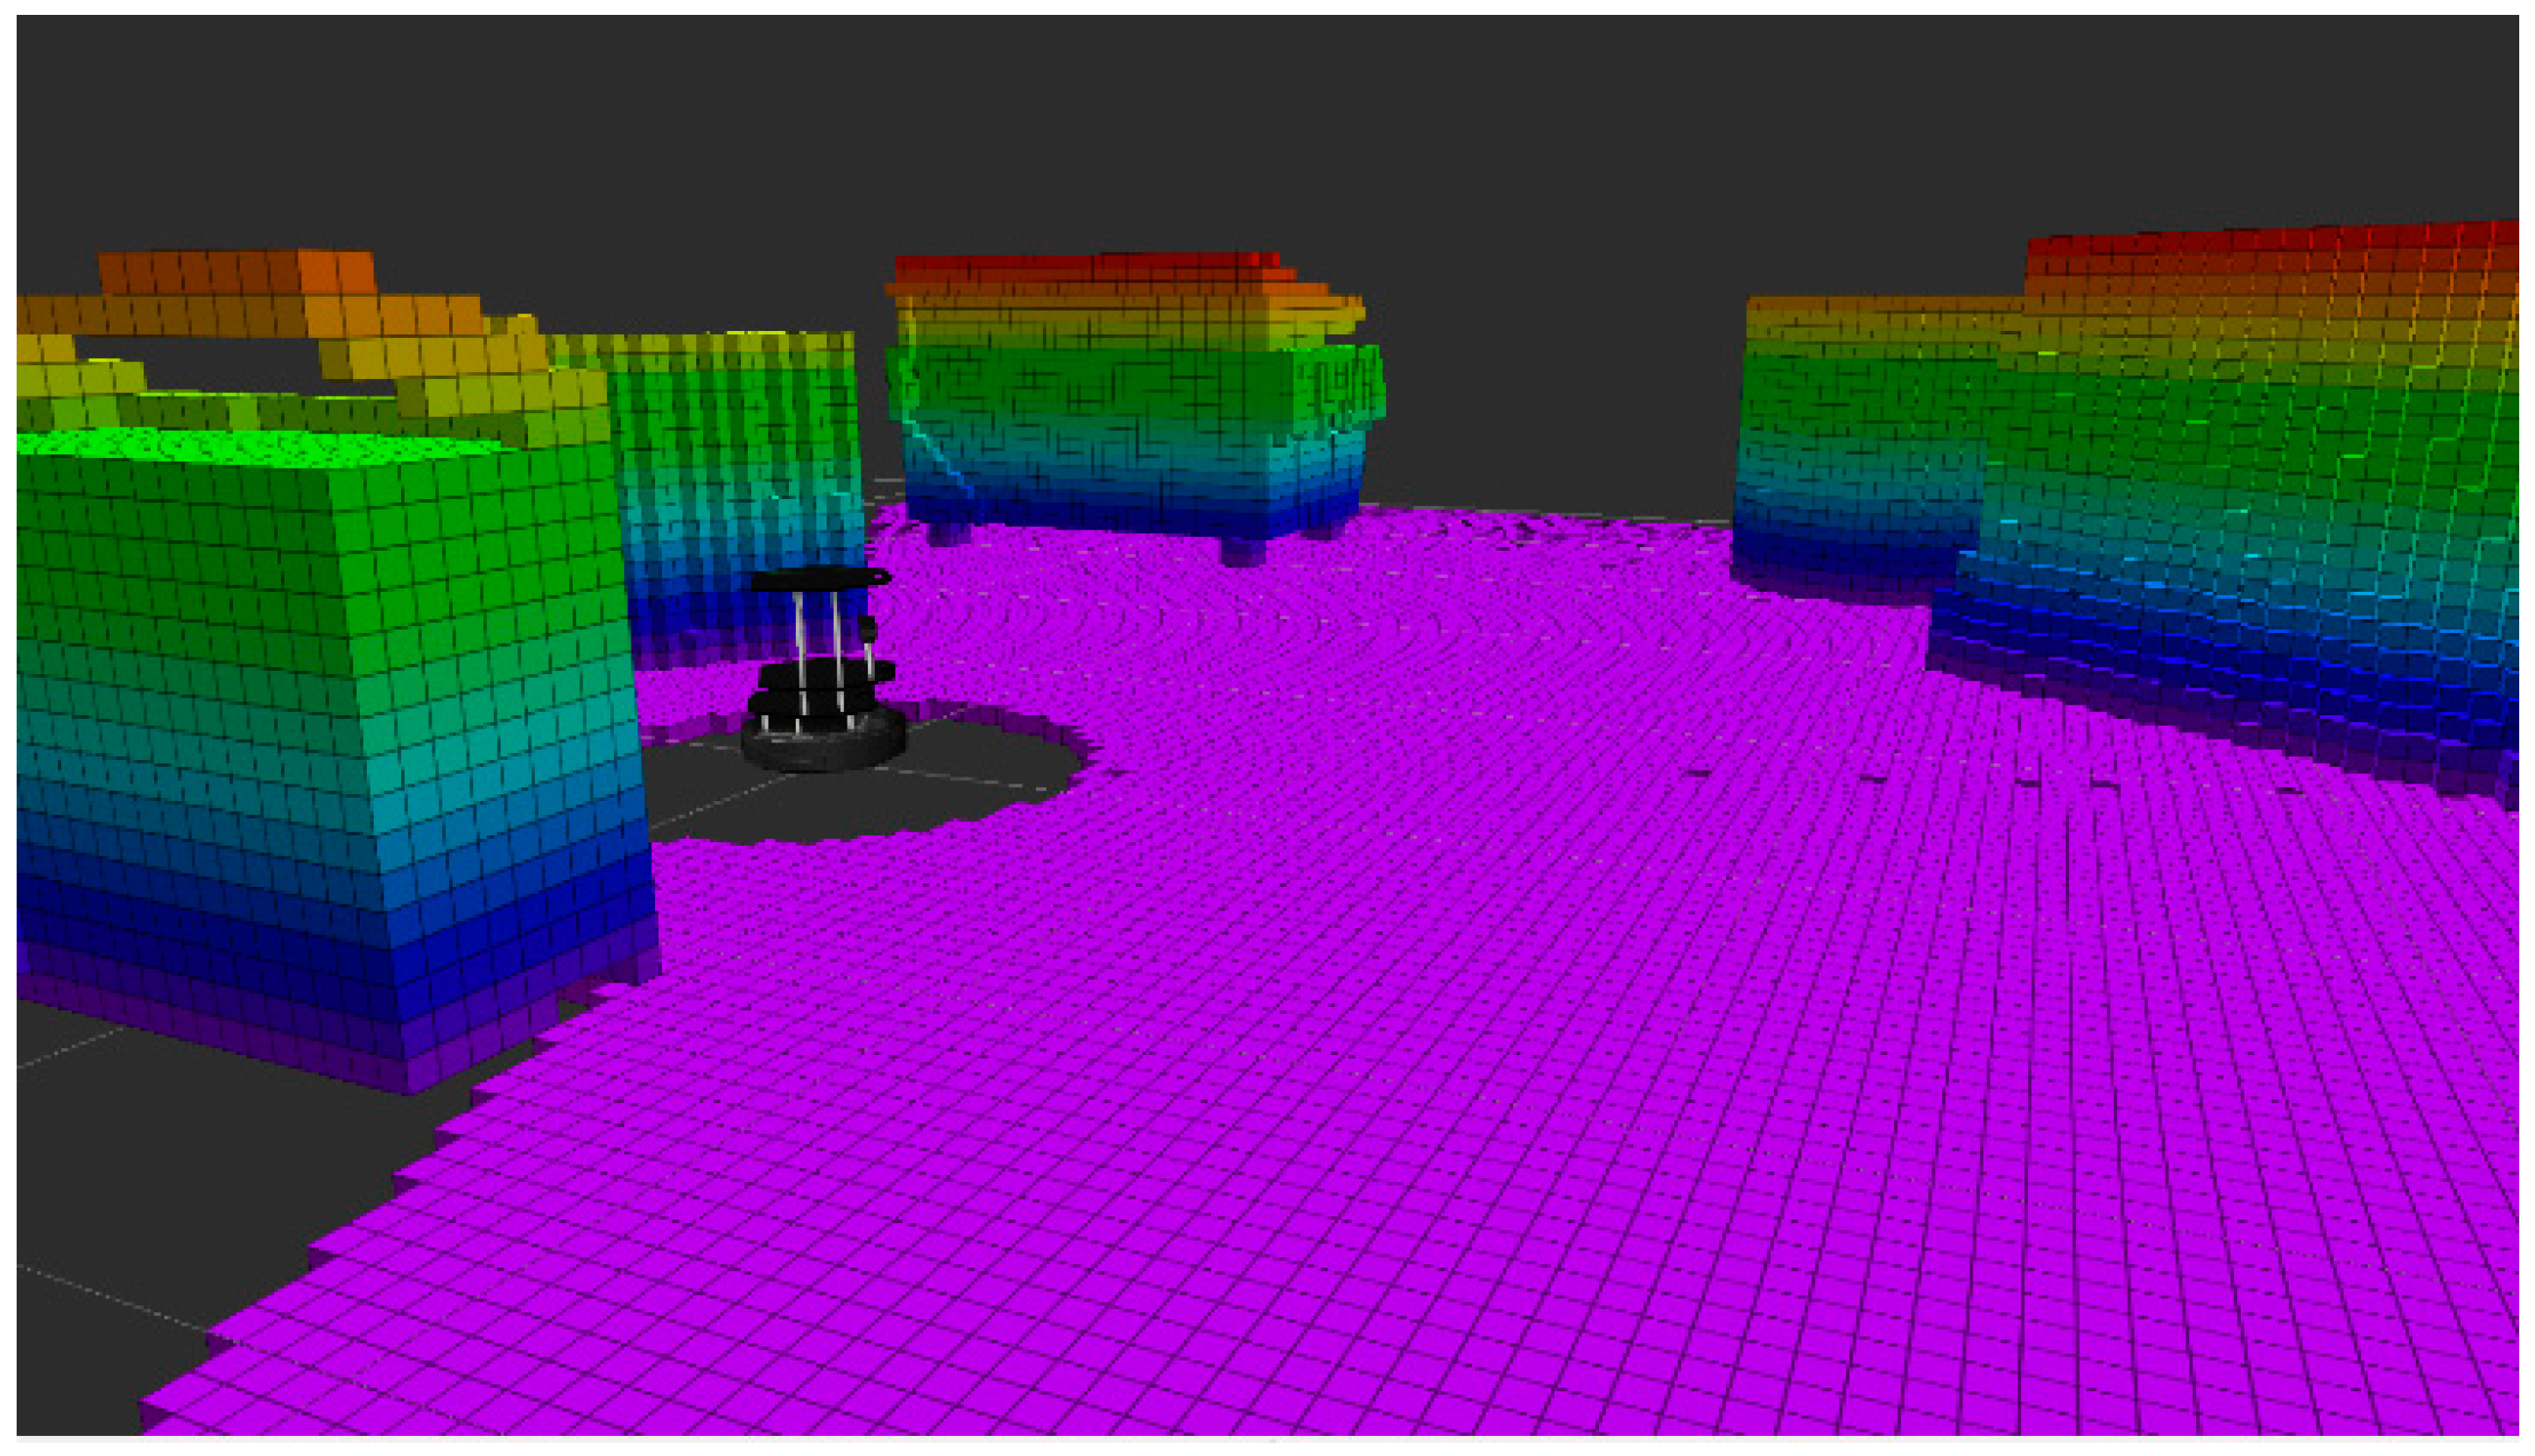
\includegraphics[scale=0.8]{turtle}\\
		3D map generated using octomap and turtlebot
\end{center}
		
\end{frame}

\begin{frame}{Task Accomplished}
Link for the video demonstartion of 
\href{https://youtu.be/W7t_BQyy5vk}{Emulating AR Drone 2.0 in Rviz}\\
Link for the video demonstartion of \href{https://youtu.be/Q2GwBIR4_pk}{Aligning AR Drone 2.0 to ArUco marker}\\

\end{frame}

\section{Challenges Faced}
\begin{frame}{Challenges Faced}
	\begin{itemize}
		\item Balaji Gorantla
        \begin{itemize}
        	\item Understanding Linux, Python, ROS.
            \item Understanding the octomap library.
            \item Tuning 4 sets of PID for aligning the drone to an ArUco marker.
        \end{itemize}
        \item Ridhwan Luthra
        \begin{itemize}
            \item Tuning 4 sets of PID for aligning the drone to an ArUco marker.
        \end{itemize}
	\end{itemize}
\end{frame}

\section{Future Plans}
\begin{frame}{Future Plans}
	%\begin{itemize}
		%\item Autonomously Navigate the drone from one point to another.
		\begin{center}
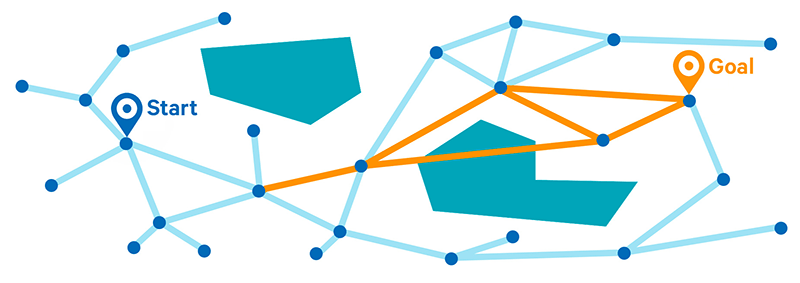
\includegraphics[scale=0.35]{auto_nav}\\
		Autonomously Navigate the drone from one point to another
\end{center}
	%\end{itemize}
\end{frame}


\section{Thank You}
\begin{frame}{Thank You}
\begin{center}

\includegraphics[scale=0.15]{parrot-ar-dronew_home}\\
	 THANK YOU !!!
	\end{center}
\end{frame}
\end{document}
